\section{Overview}\label{sec:overview}
To address the problem of analysis knowledge reuse, we want to introduce a method
can make the target program with semantic diversity.
The process of DCVP to protect the code follows several major steps described as follows 
(for better understanding, we will introduce our approach start from the design of virtual IS and \texttt{handlers}):

%\emph{Design of Virtual IS and Handlers:}
\paragraph{Design of Virtual IS and Handlers}
First design complete Virtual IS (virtual instruction set) according to the classification of native instructions, and then design the \texttt{handlers} that used to interpret the VI (Virtual Instruction). The details are described as section~\ref{sec:VIS-Handlers}.

%\paragraph{Native Instructions to VIs:}
\paragraph{Target Instructions Virtualization}
Extract the native instructions of key code segment from the target program, and then convert native instructions to the corresponding VIs according to designed virtual IS. The details are described as section~\ref{sec:NI-VI}.

%\paragraph{VIs to Bytecode:}
\paragraph{Generate Diversified Bytecode Program}
Convert the virtual instructions into a diversified bytecode program by using a special encoding schemes. Each protected code region will be partitioned into multiple segments where the mapping of opcodes and their semantics are randomized in different ways in different segments.
Then generate multiple sets of \texttt{handlers} that with equivalent functions but different forms makes each partition has unique interpretation procedures. DCVP will also adopt some anti-taint analysis techniques to protect the core components from taint analysis.
The details are described as section~\ref{sec:VI-Bytecode}.


\paragraph{PE Refactoring}
%DCVP will convert all of the critical instructions into bytecode program that can only be interpreted by the system itself.
Finally the bytecode program and other VM components (such as, \texttt{VMloop}, \texttt{VMcontext} et al.) are assembled into the target program through binary rewriting.



\section{Virtual Instruction Set and Handlers}\label{sec:VIS-Handlers}
As the basis of a VM-based obfuscation system, virtual IS and the \texttt{handlers} should be the first considerations when designing such an system. The challenge lies in devising a feature-complete virtual IS that is Turing-equivalent to native IS, which means that any native instructions could be substituted with the virtual instructions. Virtual instructions ultimately will be executed by the hand-crafted \texttt{handlers}; these \texttt{handlers} are written in native instructions.

There are two main VM architectures: stack-based, and register-based. Examples of stack-based virtual machines are the Java Virtual Machine and the .Net CLR, and examples of register-based virtual machines are the Lua VM, and the Dalvik VM. In this paper, we choose stack-based architecture for the VM-based obfuscation system for the following reasons:
\begin{itemize}
  \item In a stack-based VM, operations are carried out with the help of stack, where operands and results of operations are stored. This simplifies the addressing of operands and ultimately simplifies the implementation of \texttt{handlers}.
  \item The process of converting native x86 instructions to virtual instructions is simpler.
  \item Stack-based VMs require more virtual instructions for a given computation; this makes the instructions more complex and conforms to our objective of impeding reverse analysis.
\end{itemize}

To devise a virtual IS that is Turing-equivalent to the native IS, one naive approach is devising a virtual instruction for every single native instruction. However, this results in a very large size of handlers. As the basic idea of stack-based VMs implies, a native operation are carried out or virtualized by virtual instructions in a three-phase fashion: pushing operands into the stack, executing the aimed operation, and storing the result into the virtual context. Therefore, it is sufficient for the virtual IS to include the following instructions:
\begin{itemize}
  \item \texttt{load} instructions and \texttt{store} instructions for data transfers. \texttt{load} instructions are for pushing operands into stack, and \texttt{store} instructions are for popping results out of the stack and store the results into the virtual context.
  \item Arithmetical and logical instructions. The variants of these kind of instructions are much smaller than their native ones, as the addressing mode of operands is simpler and uniform, i.e., stack-based addressing.
  \item Branch instructions for changing the control flow of bytecode program.
\end{itemize}

Other instructions that are not included in the above categories are defined as special virtual instruction - \texttt{undef}, which we will discuss later. We first discuss the different formats of these instructions and how to implement the handlers of them.

\begin{table}[]
\renewcommand{\arraystretch}{1.1}
\tbl{The Virtual Instructions and Corresponding Handlers of \texttt{load} and \texttt{store}.\label{tab:load}}{

\begin{tabular}{|l|l|}
\hline
VI              & Handler                     \\ \hline \hline
\texttt{load\underline{ }r reg}     & \texttt{movzx eax, byte [VPC]} \textit{;get vr index}     \\
                & \texttt{add VPC, 1}                  \\
                & \texttt{push dword [VMcontext+eax*4]}                  \\ \hline
\texttt{load\underline{ }r8h reg}   & \texttt{movzx eax, byte [VPC]} \emph{;get vr index}      \\
                & \texttt{add VPC, 1}                  \\
                & \texttt{movzx eax, byte [VMcontext+eax*4+1]}              \\
                & \texttt{push eax}                                      \\ \hline
\texttt{load\underline{ }m mem}     & \texttt{mov eax, dword [VPC]} \emph{;get memory addr}            \\
                & \texttt{add VPC, 4}                  \\
                & \texttt{push dword [eax]}                              \\ \hline
\texttt{load\underline{ }i8 imm8}     & \texttt{movzx eax, byte [VPC]} \emph{;get 8-bit imm value}            \\
                & \texttt{add VPC, 1}                  \\
                & \texttt{push eax}                                      \\ \hline
\texttt{load\underline{ }i16 imm16}     & \texttt{movzx eax, word [VPC]} \emph{;get 16-bit imm value}            \\
                & \texttt{add VPC, 2}                  \\
                & \texttt{push eax}                                      \\ \hline
\texttt{load\underline{ }i32 imm32}     & \texttt{mov eax, dword [VPC]} \emph{;get 32-bit imm value}            \\
                & \texttt{add VPC, 4}                  \\
                & \texttt{push eax}                                      \\ \hline
\texttt{load\underline{ }ms}        & \texttt{pop eax}                                       \\
                & \texttt{push dword [eax]}                              \\ \hline
\texttt{store\underline{ }r reg}    & \texttt{movzx eax, byte [VPC]} \emph{;get vr index}     \\
                & \texttt{add VPC, 1}                  \\
                & \texttt{pop dword [VMcontext+eax*4]}                   \\ \hline
\texttt{store\underline{ }r8h reg}  & \texttt{movzx eax, byte [VPC]} \emph{;get vr index}     \\
                & \texttt{add VPC, 1}                  \\
                & \texttt{pop edx}                                       \\
                & \texttt{mov byte [VMcontext+eax*4+1], dl}                \\ \hline
\texttt{store\underline{ }m mem}    & \texttt{mov eax, dword [VPC]} \emph{;get memory addr}               \\
                & \texttt{add VPC, 4}                  \\
                & \texttt{pop dword [eax]}                               \\ \hline
\texttt{store\underline{ }ms}       & \texttt{pop eax}                                       \\
                & \texttt{pop ebx}                                       \\
                & \texttt{mov dword [eax], ebx}                          \\ \hline
\end{tabular}
}
\begin{tabnote}
\Note{Note:}{In the table, \texttt{reg} means register, \texttt{mem} memory address, \texttt{imm} immediate value, and \texttt{vr} virtual register. \texttt{VPC} is short for Virtual Program Counter and represents the address of the next bytecode instruction to interpret.}
\end{tabnote}
\end{table}


\subsection{"\texttt{load}" and "\texttt{store}" Instructions}
\texttt{load} and \texttt{store} instructions are used for preparing operands and storing the results of operations. They are used in the first and third phases of virtualizing a native instruction. In our virtual IS, they are the only ones that have operands. For a \texttt{load} instruction, the operand could be a virtual register, a memory addresses, or an immediate value, and for a \texttt{store} instruction, the operand is a virtual register or a memory address. Virtual registers are stored in the virtual context, i.e., the \texttt{VMcontext}. A naive construction of \texttt{VMcontext} is simply copying the values of native registers into the \texttt{VMcontext}. But the mapping between the virtual registers and the native registers is not necessarily one-to-one. To further impede the reverse analysis, the mapping mechanism could be made purposely more complex, as NISLVMP \cite{wang2013nislvmp} does. In this section, we only consider the one-to-one mapping between the virtual registers and the native ones.



Besides the operand type, the operand size matters as well. In x86 architecture, the size of an operand could be 8-bit, 16-bit, and 32-bit. For example, given a memory address, the \texttt{load} instruction could fetch the first 8-bit, or the lower 16-bit value, or the entire 32-bit value that stored in that address. Therefore, it is better to design a virtual instruction for every distinct combination of operand type and size. However, in x86 architecture, \texttt{push} and \texttt{pop} operations do not support 8-bit operations. We decide to delay distinguishing different size operands to the second phase of virtualizing native instructions. Table \ref{tab:load} shows the virtual instructions of \texttt{load} and \texttt{store} and their corresponding \texttt{handlers}. In table \ref{tab:load}, there exists four special virtual instructions: \texttt{load\underline{ }r8h} and \texttt{store\underline{ }r8h} are used when we encounter an operation that manipulate the second least significant byte of a register, i.e., \texttt{ah}, \texttt{dh}, \texttt{ch}, \texttt{bh}. \texttt{load\underline{ }ms} and \texttt{store\underline{ }ms} have no operands and are used to process instructions with indirect memory addressing mode (memory address is stored in a register or presented as an expression). An example in table \ref{tab:native2virtual} illustrates the situation of using of \texttt{load\underline{ }ms}.

\begin{table}[!t]
\renewcommand{\arraystretch}{1.1}
\tbl{The Virtual Instructions and Handlers of \texttt{add} Virtual Instructions.\label{tab:arithmetic}}{
\begin{tabular}{|l|l|}
\hline
VI             & Handler  \\ \hline \hline
\texttt{add8}   & \texttt{pop eax}              \\
                & \texttt{add \textit{byte} [esp], al}   \\ \hline
\texttt{add16}  & \texttt{pop eax}              \\
                & \texttt{add \textit{word} [esp], ax}   \\ \hline
\texttt{add32}  & \texttt{pop eax}              \\
                & \texttt{add \textit{dword} [esp], eax} \\ \hline
\end{tabular}}
\begin{tabnote}
\Note{Note:}{Since the operations of these instructions could be 8-bit, 16-bit, or 32-bit, we design a virtual instruction for each of the operations of different operand size.}
\end{tabnote}
\end{table}


\subsection{Arithmetical and Logical Instructions}
Arithmetical and logical virtual instructions are used to execute the aimed operations and they need not to worry about operands, since their operands have been pushed into the stack by \texttt{load} instructions. However, as we said before, these instructions must consider the size of the operands. These instructions are in similar forms and we take \texttt{add} operation as an example to illustrate. Table~\ref{tab:arithmetic} lists the virtual instructions and handling procedures of \texttt{add} operation. Since the operations of these instructions could be 8-bit, 16-bit, or 32-bit, we design a virtual instruction for each of the operations of different operand size.




\subsection{Branch Instructions}
In native IS, the commonly used branch instructions include \texttt{jmp}, \texttt{jcc} (conditional jump), \texttt{call}, and \texttt{retn}. It is a big challenge to virtualize these instructions, since they have many different variants and each of these variants needs a virtual instruction. Considering the destination of a jump (branch) instruction, if its destination also resides in the critical code, we call it an \emph{inner jump}; otherwise, we call it an \emph{outer jump}. Figure \ref{fig:jump} illustrates these two kinds of branch instructions. In DCVP, we ignore the situation where the destination of a branch instruction outside the critical code resides in the critical code, the start instruction of the critical code excluded. This situation will not occur if the critical code to be protected is well-structured.

\begin{figure}[!ht]
\centering
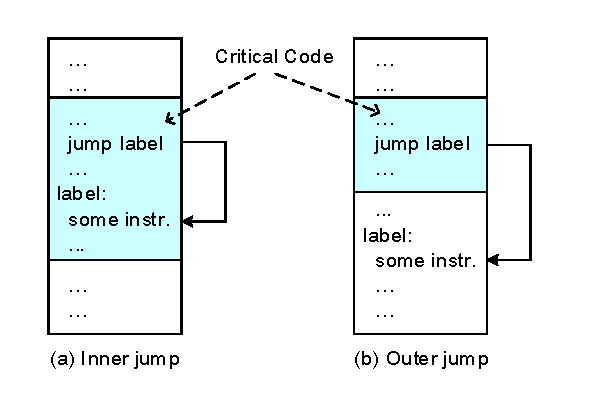
\includegraphics[width=0.45\columnwidth]{fig/jump.pdf}
\caption{The destination of a branch instruction could be in the critical code or outside the critical code. Branch instructions include \texttt{jmp}, \texttt{jcc}, \texttt{call}, and \texttt{retn}.}
\label{fig:jump}
\end{figure}

Besides the location of the destination instruction, we should also consider if the destination of a branch instruction can be determined statically. From this point of view, the branch instructions can be divided into two categories: one is \emph{direct branches}, whose destinations are calculated in a PC (Program Counter)-relative mode and can be calculated statically. The other is \emph{indirect branches}, whose destinations are stored in registers or memories. Their destinations are undefined statically and are determined at runtime. Table \ref{tab:controltransfers} classifies different forms of \texttt{jmp/jcc/call/retn} instructions considering the above two categories.

\begin{table}[h]
\renewcommand{\arraystretch}{1.1}
\tbl{Examples of Direct and Indirect Branches.\label{tab:controltransfers}}{
\begin{tabular}{|l|l|}
\hline
Direct Branches   & \texttt{jmp rel8/16/32}   \\
                           & \texttt{jcc rel8/16/32}   \\
                           & \texttt{call rel16/32}    \\ \hline
Indirect Branches & \texttt{jmp reg32/mem32}  \\
                           & \texttt{call reg32/mem32} \\
                           & \texttt{retn}             \\ \hline
\end{tabular}}
\begin{tabnote}
\Note{Note:}{In this table, \texttt{rel} means a PC-relative address. The numbers (8, 16, and 32) are the size (in bit) of the operands.}
\end{tabnote}
\end{table}


\textbf{Direct Branches}. Since \texttt{jmp} instructions are the basis of the other branch instructions, we elaborate on the introduction of the virtual instructions and handlers of \texttt{jmp} instructions. As we have illustrated, the destination of a direct \texttt{jmp} instruction can be calculated statically. If the destination instruction of the \texttt{jmp} instruction resides in the critical code, the \texttt{jmp} is a \textit{direct inner} \texttt{jmp}; otherwise a \textit{direct outer} \texttt{jmp}. We designate virtual instructions for both of them, \texttt{jmp\underline{ }di} for the former, and \texttt{jmp\underline{ }do} for the latter. For \textit{direct inner} \texttt{jmp}, it is able to obtain the corresponding bytecode instruction address of its native destination instruction during protection. Therefore, we set that bytecode instruction address as the operand of \texttt{jmp\underline{ }di}, which is pushed into stack by \texttt{load\underline{ }i}. The handler of \texttt{jmp\underline{ }di} fetches the address from stack and assigns it to VPC (Virtual Program Counter). For \textit{direct outer} \texttt{jmp}, we just need to jump to that destination instruction. Prior to that, we should restore the native context. Therefore, the operand of \texttt{jmp\underline{ }do} is the address of the native destination instruction. Table \ref{tab:jmp} presents the above two virtual instructions of \textit{direct} \texttt{jmp} and their handlers.

\begin{table}[!ht]
\renewcommand{\arraystretch}{1.1}
\tbl{The Virtual Instructions and Handlers of \texttt{jmp} Instructions.\label{tab:jmp}}{ %\texttt{jmp\underline{ }di} is for \textit{direct inner} \texttt{jmp} and \texttt{jmp\underline{ }do} for \textit{direct outer} \texttt{jmp}.}
\begin{tabular}{|c|l|}
\hline
VI                           & Handler      \\ \hline \hline %\raisebox{1.0ex}[0pt]{Handler}\\ \hline \hline
\texttt{jmp\underline{ }di}  & \emph{;operand: addr of the dest. bytecode instr.}        \\
                             & \texttt{pop eax} \emph{;get operand}                \\
                             & \texttt{mov VPC, eax}                                                \\ \hline
\texttt{jmp\underline{ }do}  & \emph{;operand: addr of the dest. native instr.}          \\
                             & \texttt{pop [mem]} \emph{;get operand}               \\
                             & \texttt{...} \emph{;restore native context}                         \\
                             & \texttt{jmp dword [mem]}                                             \\ \hline
\end{tabular}}
\begin{tabnote}
\Note{Note:}{\texttt{jmp\underline{ }di} is for \textit{direct inner} \texttt{jmp} and \texttt{jmp\underline{ }do} for \textit{direct outer} \texttt{jmp}.}
\end{tabnote}
\end{table}

\texttt{jcc} and \textit{direct} \texttt{call} instructions are similar to \textit{direct} \texttt{jmp}. \texttt{jcc} has many different kinds of instructions for different conditions, and each needs a specific virtual instruction. In the \texttt{handlers}, some extra instructions are needed to check the state of the conditions and decide to jump or not. \texttt{call} instructions can be considered as a \texttt{push} instruction followed by a \texttt{jmp} instruction. The \texttt{push} instruction pushes the return address into the stack and the \texttt{jmp} instruction jumps to the address of the subroutine.


\textbf{Indirect Branches}. Since it is difficult to obtain the address of an indirect branch, we cannot decide whether the branch is an inner one or an outer one. One solution is to delay the decision until runtime. In such case, however, the implementation of the handler is complex. Hence, for these instructions, instead of using a similar idea as that for \textit{direct branches}, we use a special virtual instruction \texttt{undef}, which will be introduced later.

\subsection{Other Instructions}
The above three categories cover the commonly used instructions. Although the other native instructions are rarely used, such as \texttt{bts}, \texttt{enter}, \texttt{int n}, and \texttt{out}, our native IS should consider them too. For these instructions, we define a special virtual instruction - \texttt{undef}. At runtime, when encountering such an instruction, it first restores the native context and exits the VM. Then, it executes that native instruction in native context and finally re-enters the VM and continues to execute the left bytecode instructions. The \textit{indirect branches} are also processed in this way.

\begin{table}[!t]
\renewcommand{\arraystretch}{1.1}
\tbl{Examples of Native Instructions and Their Corresponding Virtual Instructions.\label{tab:native2virtual}}{
\begin{tabular}{|l|l|}
\hline
Native Instr. & VI                          \\ \hline \hline
\texttt{mov eax, ebx}            & \texttt{load\underline{ }r 3}         \\
                                 & \texttt{store\underline{ }r 0}        \\ \hline
\texttt{mov eax, dword [esi+4]}  & \texttt{load\underline{ }r 6}         \\
                                 & \texttt{load\underline{ }i32 4}        \\
                                 & \texttt{add32}             \\
                                 & \texttt{load\underline{ }ms}           \\
                                 & \texttt{store\underline{ }r 0}        \\  \hline
\texttt{add eax, edx}            & \texttt{load\underline{ }r 0}         \\
                                 & \texttt{load\underline{ }r 2}         \\
                                 & \texttt{add32}             \\
                                 & \texttt{store\underline{ }r 0}        \\ \hline
\texttt{jmp 4020a8h}             & \texttt{load\underline{ }i32 42a583h}   \\
(direct inner jump)              & \texttt{jmp\underline{ }di}           \\ \hline
\end{tabular}}
\begin{tabnote}
\Note{Note:}{\texttt{42a583h} is the bytecode instruction address that corresponds to the native instruction at \texttt{4020a8h}.}
\end{tabnote}
\end{table}
